\documentclass[compress,12pt]{beamer}

\usetheme{Arguelles}
\usepackage{graphicx}
\usepackage{caption}
%\usepackage[spanish,es-noshorthands]{babel}
\usepackage{babel} 
\usepackage[pages=some]{background}
\usepackage{tikz}
\usepackage{tikz-cd}
\usepackage{amsmath,amssymb,latexsym,amscd} 
\usepackage[all,cmtip]{xy}
\usepackage{fancyhdr}
\usepackage{mathalfa}
\usepackage{mathrsfs}
\usetikzlibrary{babel}
\usepackage{hyperref}
\usepackage{ragged2e}
\usepackage{wasysym}
\usepackage{tikz}
\usetikzlibrary{arrows.meta,calc,positioning,overlay-beamer-styles,shadows.blur}
%\hypersetup{colorlinks=true,linkcolor=blue,citecolor=brown,linktocpage=true,pagebackref=true,hyperindex=true}
\pagenumbering{arabic}

\DeclareMathOperator{\op}{op}
\DeclareMathOperator{\pt}{pt}
\DeclareMathOperator{\spec}{spec}
\DeclareMathOperator{\Fit}{Fit}
\DeclareMathOperator{\Pth}{P}
\DeclareMathOperator{\Frm}{Frm}
\DeclareMathOperator{\Top}{Top}
\DeclareMathOperator{\Ord}{Ord}
\DeclareMathOperator{\Obj}{Obj}
\DeclareMathOperator{\Hom}{Hom}

\title{Modificaciones de parches}
\subtitle{y algunos axiomas de separación en la topología sin puntos}
%\event{58° Congreso Nacional de la SMM}
\date{\today}
\author{Juan Carlos Monter Cortés \\ Director: Dr. Luis Ángel Zaldívar Corichi}
\institute{Universidad de Guadalajara}
%\email{juan.monter2902@alumnos.udg.mx}

%\homepage{www.mywebsite.com}
%\github{username}

\begin{document}

\frame[plain]{\titlepage}


\begin{frame}{La construcción de parches}
\centering
\resizebox{\textwidth}{!}{%
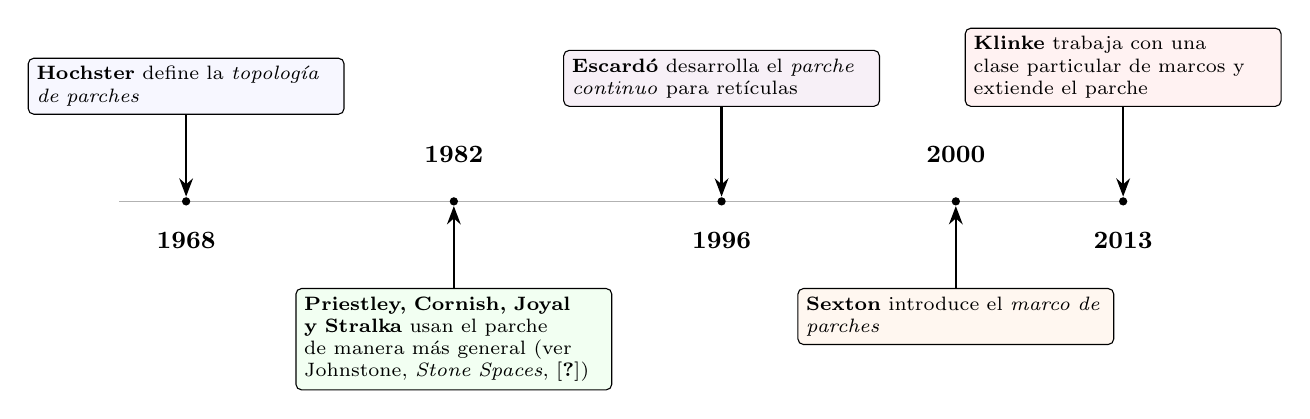
\begin{tikzpicture}[
  x=0.85cm, y=1cm,
  >=Stealth,
  year/.style={font=\small\bfseries},
  base/.style={
    draw, rounded corners=2pt, fill=white, align=left, inner sep=3pt,
    font=\scriptsize, text width=3.8cm
  },
  E1968/.style={base, fill=blue!3},
  E1982/.style={base, fill=green!5},
  E1996/.style={base, fill=violet!6},
  E2000/.style={base, fill=orange!6},
  E2013/.style={base, fill=red!5},
  tick/.style={circle, fill, minimum size=3pt, inner sep=0pt},
  axis/.style={line width=0.6pt, gray!60}
]

% --- Eje base
\draw[axis] (0,0) -- (15,0);

% --- Coordenadas
\coordinate (p68) at (1,0);
\coordinate (p82) at (5,0);
\coordinate (p96) at (9,0);
\coordinate (p00) at (12.5,0);
\coordinate (p13) at (15,0);

% --- Años (1968, 1996 abajo; 1982, 2000, 2013 arriba)
\node[tick, visible on=<1->] at (p68) {};
\node[year, visible on=<1->] at ($(p68)+(0,-0.5)$) {1968};

\node[tick, visible on=<2->] at (p82) {};
\node[year, visible on=<2->] at ($(p82)+(0,0.6)$) {1982};

\node[tick, visible on=<3->] at (p96) {};
\node[year, visible on=<3->] at ($(p96)+(0,-0.5)$) {1996};

\node[tick, visible on=<4->] at (p00) {};
\node[year, visible on=<4->] at ($(p00)+(0,0.6)$) {2000};

\node[tick, visible on=<5->] at (p13) {};
\node[year, visible on=<5->] at ($(p13)+(0,-0.5)$) {2013};

% --- Eventos alternados
\node[E1968, anchor=south, visible on=<1->] (e1968) at ($(p68)+(0,1.1)$)
  {\textbf{Hochster} define la \emph{topología de parches}};

\node[E1982, anchor=north, visible on=<2->] (e1982) at ($(p82)+(0,-1.1)$)
  {\textbf{Priestley, Cornish, Joyal y Stralka} usan el parche de manera más general (ver Johnstone, \emph{Stone Spaces}, \cite{P.T.})};

\node[E1996, anchor=south, visible on=<3->] (e1996) at ($(p96)+(0,1.2)$)
  {\textbf{Escard\'o} desarrolla el \emph{parche continuo} para retículas};

\node[E2000, anchor=north, visible on=<4->] (e2000) at ($(p00)+(0,-1.1)$)
  {\textbf{Sexton} introduce el \emph{marco de parches}};

\node[E2013, anchor=south, visible on=<5->] (e2013) at ($(p13)+(0,1.2)$)
  {\textbf{Klinke} trabaja con una clase particular de marcos y extiende el parche };

% --- Flechas verticales
\draw[->, thick, visible on=<1->] (e1968.south) -- ($(p68)+(0,0.06)$);
\draw[->, thick, visible on=<2->] (e1982.north) -- ($(p82)+(0,-0.06)$);
\draw[->, thick, visible on=<3->] (e1996.south) -- ($(p96)+(0,0.06)$);
\draw[->, thick, visible on=<4->] (e2000.north) -- ($(p00)+(0,-0.06)$);
\draw[->, thick, visible on=<5->] (e2013.south) -- ($(p13)+(0,0.06)$);

\end{tikzpicture}%
% end resizebox
}
\end{frame}

\begin{frame}[fragile]{Teoría de marcos}
\[
\Frm= \left\{ \begin{array}{lc} \Obj: & (A, \leq, \wedge, \bigvee, 1, 0) \\ \\ \mbox{Flechas:} & f\colon A\to B  \end{array} \right.
\]

Para $S\in \Top$,
\[
(\mathcal{O}S, \subseteq, \cap, \bigcup, S, \emptyset)\in \Frm
\]
Además,,
\[
\begin{tikzcd}
\Top \arrow[rr, "\mathcal{O}( \_ )", bend left] & \perp & \Frm \arrow[ll, "\pt( \_ )", bend left]
\end{tikzcd}
\]
es una adjunción.
\end{frame}

\begin{frame}{Espacio de parches}
    $^pS=(S, \mathcal{O}^pS)$, donde $\mathcal{O}^pS$ está generado por
    \[
    \mbox{pbase}=\{U\cap Q'\mid U\in \mathcal{O}S, Q\in \mathcal{Q}S\}
    \]
\begin{block}{Definición}
$S\in \Top$ es \textbf{empaquetado} si todo subconjunto compacto (saturado) es cerrado
\end{block}
\[
S \mbox{ es empaquetado}\quad\iff\quad ^pS=S
\]

\[
T_2\Rightarrow \mbox{empaquetado}\Rightarrow T_1
\]
\end{frame}

\begin{frame}{Parche trivial}
Por el \emph{Teorema de Hoffman-Mislove}\footnote{\textbf{Teo:} Existe una correspondencia biyectiva entre $F\in A^\wedge$ y $Q\in \mathcal{Q}S$}
\[
\mbox{Pbase}=\{u_a\wedge v_F\mid a\in A, F\in A^\wedge\}
\]
\begin{block}{Definición}
\begin{enumerate}
    \item El \textbf{marco de parches} de $A\in \Frm$ $(PA)$, es el marco generado por la Pbase.
    \item $A$ es \textbf{parche trivial} si $A\simeq PA$.
\end{enumerate}
\end{block}

\footnotetext[0]{$F\in A^\wedge$ si $F$ es un filtro en $A$ y $\forall\, X\subseteq A$, con $X$ dirigido, si $\bigvee X\in F$, entonces $a\in F$ para algún $a\in X$.}
\footnotetext[0]{Para $a\in A$, $u_a(x)=a\vee x$ y $v_a(x)=(a\succ x)$ son núcleos en $A$.}
\footnotetext[0]{$v_F=f^\infty$, donde $f=\dot{\bigvee}\{v_a\mid a\in F\}$ }
\end{frame}

\begin{frame}{Marcos eficientes}
\begin{block}{Definition [\cite{R.S.3}, Def. 8.2.1]}
Let $A\in \Frm$, $F\in A^\wedge$ and $\alpha\in \Ord$ be. We say that:
\begin{enumerate}
    \item $F$ is $\alpha$-tidy if for $x\in F$, $d\vee x=1$, where
    \[
    d=d(\alpha)=f^\alpha(0).
    \]
    \item $A$ is $\alpha$-tidy if every $F\in A^\wedge$ is $\alpha$-tidy.
    \item $A$ is \textbf{tidy} if it is $\alpha$-tidy for some $\alpha\in \Ord$.
\end{enumerate}
\end{block}

\begin{block}{Proposition [\cite{R.S.3}, Lemma 8.2.2]}
\[
    A \mbox{ is tidy}\quad \iff\quad A \mbox{ is patch trivial}.
\]
\end{block}
\end{frame}

\begin{frame}[plain,standout]
      \centering{
      \Huge{Objectives}}
      \begin{enumerate}
        \item Understand tidy frames in more detail.
        \item To explore the relationship with some separation axioms in $\Frm$.
        \item Provide tools to study the tidy frames.
        \item Give examples.
      \end{enumerate}
\end{frame}

\begin{frame}[fragile]{Separation axioms in Frm}
\[\begin{tikzcd}
	&& {\mathbf{(reg)}} \\
	{\mathbf{(fit)}} && {\mathbf{(sH)}} && {\mathbf{(H)}+\mathbf{(sfit)}} \\
	{\mathbf{(sfit)}} && {T_1} && {\mathbf{(H)}}
	\arrow[Rightarrow, from=1-3, to=2-1]
	\arrow[Rightarrow, from=1-3, to=2-3]
	\arrow[Rightarrow, from=1-3, to=2-5]
	\arrow[Rightarrow, from=2-1, to=3-1]
	\arrow[Rightarrow, from=2-1, to=3-3]
	\arrow[dotted, no head, from=2-3, to=2-1]
	\arrow[dotted, no head, from=2-3, to=2-5]
	\arrow[dotted, no head, from=2-3, to=3-1]
	\arrow[Rightarrow, from=2-3, to=3-3]
	\arrow[Rightarrow, from=2-3, to=3-5]
	\arrow[Rightarrow, from=2-5, to=3-5]
	\arrow[dotted, no head, from=3-1, to=3-3]
	\arrow[Rightarrow, from=3-5, to=3-3]
\end{tikzcd}\]
\footnotetext[0]{$\forall\, a\nleq b\in A$, then }
\footnotetext[0]{\textbf{(reg):} $\exists \, x,y\in A$ such that $a\vee x=1, y\nleq b$ and $x\wedge y=0$.}
\footnotetext[0]{\textbf{(H):} $\exists\, c\in A$ such that $c\nleq a$ and $\neg c\leq b$.}
\footnotetext[0]{\textbf{(fit):} $\exists\, x,y\in A$ such that $x\vee a=1, y\nleq b$ and $x\wedge y\leq b$.}
\footnotetext[0]{\textbf{(sfit):} $\exists\, c\in A$ such that $c\vee a=1\neq c\vee b$.}
\footnotetext[0]{\textbf{(sH)} and $T_1$ are notion some different. All this can be found in \cite{J.P.2}.}
\end{frame}

\begin{frame}{Properties of the tidy frames}
This is a summary of the properties that Sexton includes in \cite{R.S.3}
\begin{itemize}
\item In the spatial case ($A=\mathcal{O}S$),
\[
\begin{split}
\mathcal{O}S \mbox{ is 0-tidy } & \iff S=\emptyset \\
\mathcal{O}S \mbox{ is 1-tidy } & \iff S \mbox{ is }T_2 \\
\mathcal{O}S \mbox{ is tidy } & \iff S \mbox{ is packed and stacked}.
\end{split}
\]

\item For $A\in \Frm$ arbitrary
\[
\begin{split}
A\mbox{ is }\mathbf{(reg)} & \Rightarrow A \mbox{ is tidy}\\
A\mbox{ is }\mathbf{(fit)} & \Rightarrow A \mbox{ is tidy}\\
A\mbox{ is tidy } & \Rightarrow A\mbox{ is } T_1
\end{split}
\]
\end{itemize}
\end{frame}


\End

\section*{\textsc{Referencias}}
\begin{frame}[allowframebreaks]
\frametitle{Bibliografía}
\begin{thebibliography}{20}\markboth{Bibliografía}{Bibliografía}

\bibitem{P.T.} P. T. Johnstone, \textit{Stone spaces}, Cambridge Studies in Advanced Mathematics, vol. 3, Cambridge University Press, Cambridge, 1982. MR 698074

\bibitem{J.M.} J. Monter; A. Zaldívar, \textit{El enfoque locálico de las reflexiones booleanas: un análisis en la categoría de marcos} [tesis de maestría], 2022. Universidad de Guadalajara.

\bibitem{P.S.} J. Paseka and B. Smarda, \textit{$ T_2 $-frames and almost compact frames.} Czechoslovak Mathematical Journal (1992), 42(3), 385-402.

\bibitem{J.P.} J. Picado and A. Pultr, \textit{Frames and locales: Topology without points}, Frontiers in Mathematics, Springer Basel, 2012.

\bibitem{J.P.2} J. Picado and A. Pultr, \textit{Separation in point-free topology}, Springer, 2021.

\bibitem{R.S.} RA Sexton, \textit{A point free and point-sensitive analysis of the patch assembly}, The University of Manchester (United Kingdom), 2003.

\bibitem{R.S.2} RA Sexton, \textit{Frame theoretic assembly as a unifying construct}, The University of Manchester (United Kingdom), 2000.

\bibitem{R.S.3} RA Sexton and H. Simmons, \textit{Point-sensitive and point-free patch constructions}, Journal of Pure and Applied Algebra \textbf{207} (2006), no. 2, 433-468.

\bibitem{H.S.} H. Simmons, \textit{An Introduction to Frame Theory}, lecture notes, University of Manchester. Disponible en línea en \url{https://web.archive.org/web/20190714073511/http://staff.cs.manchester.ac.uk/~hsimmons}.

\bibitem{H.S.R} H. Simmons, \textit{Regularity, fitness, and the block structure of frames.} Applied Categorical Structures 14 (2006): 1-34.

\bibitem{H.S.4} H. Simmons, \textit{The lattice theoretic part of topological separation properties}, Proceedings of the Edinburgh Mathematical Society, vol.~21, pp.~41--48, 1978.

\bibitem{H.S.V} H. Simmons, \textit{The Vietoris modifications of a frame}. Unpublished manuscript (2004), 79pp., available online at http://www. cs. man. ac. uk/hsimmons.

\bibitem{A.W.} A. Wilansky, \textit{Between T1 and T2}, MONTHLY (1967): 261-266.

\bibitem{A.Z.} A. Zaldívar, \textit{Introducción a la teoría de marcos} [notas curso], 2025. Universidad de Guadalajara.
\end{thebibliography}
\end{frame}


\end{document}